\documentclass[times,twocolumn,final]{elsarticle}

\usepackage{cag}
\usepackage{framed,multirow}

\usepackage{amssymb}
\usepackage{latexsym}

\usepackage{url}
\usepackage{xcolor}
\definecolor{newcolor}{rgb}{.8,.349,.1}

%\usepackage{hyperref}

\usepackage[switch,pagewise]{lineno} %Required by command \linenumbers below

\usepackage{xspace}
\usepackage{verbatim}

\usepackage{listings}
\lstdefinelanguage{ceu}{%
  language=C,
  morekeywords={%
    @const, @pure, @safe, CHAN, FOREVER, PAR, PROC, SIGNAL, abort, and,
    await, bool, call, class, data, define, deterministic, do, each, else,
    emit, end, escape, event, every, finalize, hor, implementation, in,
    input, interface, loop, min, native, new, nohold, not, or, output, par,
    pool, pure, return, s, signal, spawn, tag, then, this, traverse, until,
    code, public, private,
    var, watching, when, with},
}
\lstset{
  basicstyle=\small\ttfamily,
  captionpos=b,
  columns=flexible,
  commentstyle=\rmfamily\itshape,
  escapeinside={||},
  frame=tb,
  keepspaces=true,
  keywordstyle=\bfseries,
  language=ceu,
  mathescape=true,
  numbersep=4pt,
  numberstyle=\tiny,
  %upquote=true,
}

\newcommand{\CEU}{\textsc{C\'{e}u}\xspace}
\newcommand{\locs}{\emph{locs}\xspace}
\newcommand{\code}[1] {{\small{\texttt{#1}}}}
\newcommand{\Code}[1] {{\texttt{#1}}}
\newcommand{\ax}{\code{[a]}\xspace}
\newcommand{\bx}{\code{[b]}\xspace}

\journal{Computers \& Graphics}

\begin{document}

\verso{Preprint Submitted for review}

\begin{frontmatter}

\title{Structured Synchronous Reactive Programming for Game Development
        \\ \Large{Case Study: On Rewriting Pingus from C++ to \CEU}}

%\author{Francisco Sant'Anna
        %\\ Rio de Janeiro State University, Brazil
        %\\ francisco@ime.uerj.br}

\begin{comment}
- fraquezas
    - no quantitative analysis
        - so, only for 2D, non-
- intro a Ceu
    - ssrp and ceu
    - main constructs
    - determinism, termination, cite LCTES, to appear
- acknowledgment
- authors
\end{comment}

\begin{comment}
\title{Computers and Graphics submission formatting guidelines\tnoteref{tnote1}}%
\tnotetext[tnote1]{Only capitalize first
word and proper nouns in the title.}

\author[1]{Michael \snm{Wimmer}\corref{cor1}}
\cortext[cor1]{Corresponding author: 
  Tel.: +0-000-000-0000;  
  fax: +0-000-000-0000;}
\author[1]{Joaquim \snm{Jorge}\fnref{fn1}}
\fntext[fn1]{Editor-in-Chief, Computers and Graphics Journal.}  
\author[2]{Ross \snm{Laman}}
%% Third author's email
\ead{R.Laman@elsevier.com}
\author[2]{Gail \snm{Rodney}}

\address[1]{TU Wien, Favoritenstrasse 9-11/186, 1040 Wien, Austria}
\address[2]{INESC-ID, Rua Alves Redol, 9 1000-021 Lisboa, Portugal}
\end{comment}

%\received{1 February 2017}
\received{\today}
%%%% Do not use the below for submitted manuscripts
%\finalform{28 March 2017}
%\accepted{2 April 2017}
%\availableonline{15 May 2017}
%\communicated{S. Sarkar}


\begin{abstract}
We present a qualitative case study of rewriting the video game Pingus from C++
to the structured synchronous reactive language \CEU.
%
\CEU supports reactive control-flow primitives that eliminate callbacks and let
programmers write code in direct and sequential style.
Structured reactivity helps describing complex control-flow relationships in
the game logic more concisely.
%
We show gains in productivity for six behaviors in Pingus through a qualitative
analysis of the proposed implementations in \CEU in comparison to the originals
in C++.
%
We also categorize the behaviors in four recurrent control-flow patterns that
likely apply to most games.
\end{abstract}

\begin{keyword}
%% MSC codes here, in the form: \MSC code \sep code
%% or \MSC[2008] code \sep code (2000 is the default)
%\MSC 41A05\sep 41A10\sep 65D05\sep 65D17
%% Keywords
%\KWD Computers and Graphics\sep Formatting\sep Guidelines
%C++                         \sep
%\CEU                        \sep
Control Flow                \sep
Event-Driven Programming    \sep
Game Logic                  \sep
Synchronous Reactive Programming
\end{keyword}

\end{frontmatter}

\linenumbers

\section{Introduction}

\begin{figure}
\centering
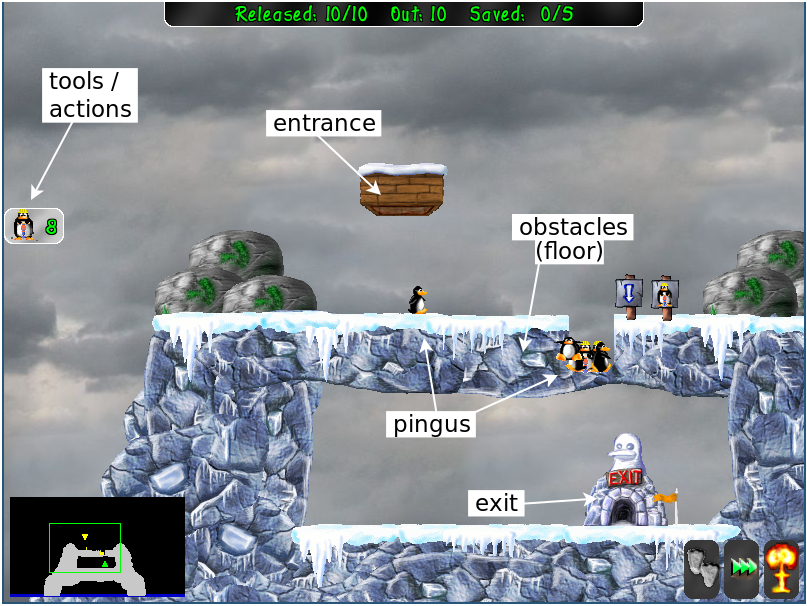
\includegraphics[width=\columnwidth]{pingus-annotations}
\caption{Pingus gameplay.
\label{fig.pingus}
}
\end{figure}

Pingus is an open-source puzzle-platform video game based on Lemmings.
The objective of the game is to guide a group of penguins through a number of
obstacles towards a designated exit (Figure~\ref{fig.pingus}).
% \footnote{Pingus gameplay video: \url{www.youtube.com/watch?v=MKrJgIFtJX0}}.
%
Pingus is developed in standard object-oriented C++, ``the lingua franca of
game development'' \cite{games.patterns}.
The codebase%
\footnote{Official Pingus repository: \url{github.com/Pingus/pingus/}}
is about 40.000 lines of code (\locs), divided into
the engine, level editor, auxiliary libraries, and the game logic itself.

According to Tim Sweeney (of Unreal Engine fame), about half the complexity in
game development resides in \emph{simulation} (aka \emph{game logic}), but
which only accounts for 10\% of the CPU budget~\cite{games.sweeney}.
%(Figure~\ref{fig.sweeney}).
%The game logic ``models the state of the game world as interacting objects
%evolve over time''.
The high development costs contrasting with the low impact on performance
appeals for alternatives with productivity in mind, especially considering that
it is the game logic that varies the most between projects.
Sweeney states that ``will gladly sacrifice 10\% of our performance for 10\%
higher productivity''.

%\begin{figure}
%\centering
%\includegraphics[width=\columnwidth]{sweeney}
%\caption{Three kinds of code~\cite{games.sweeney}.
%\label{fig.sweeney}
%}
%\end{figure}

Object-oriented games rely on the \emph{observer pattern}~\cite{games.patterns}
to handle events from the environment (e.g., key presses and timers) and also
as a notification mechanism between entities in the game logic.
%
The observers are short-lived callbacks that have to execute as fast as
possible to keep the game reactive to incoming events in real time.
%
For this reason, callbacks cannot use long-lasting locals and loops, which are
elementary capabilities of classical structured
programming~\cite{rp.deprecating,rp.rescala,sync_async.cooperative}.
%
In this sense, callbacks actually disrupt structured programming, becoming
``our generation's \emph{goto}''.%
%\footnote{``Callbacks as our Generations' \emph{goto} Statement'':
%\url{tirania.org/blog/archive/2013/Aug-15.html}}
%\footnote{``Escape from Callback Hell'':
%\url{elm-lang.org/learn/Escape-from-Callback-Hell.elm}}

In this work, we advocate structured synchronous reactive programming as a more
productive alternative for game logic development.
We present a qualitative case study of rewriting Pingus from C++ to \CEU.

\CEU~\cite{ceu.sensys13,ceu.mod15} is a Esterel-based~\cite{esterel.ieee91}
programming language that originally targets embedded soft real-time systems.
It aims to offer a concurrent, safe, and expressive alternative to C with the
characteristics that follow:
%
\begin{description}
\item [Reactive:] code only executes in reactions to events.
\item [Structured:] programs use structured control mechanisms, such as
    \code{spawn} and \code{await} (to create and suspend activities).
\item [Synchronous:] reactions run atomically and to completion on each line of
    execution, i.e., there's no implicit preemption or real parallelism.
\end{description}
%
Structured reactive programming lets developers write code in direct style,
recovering from the inversion of control imposed by event-driven
execution~\cite{rp.deprecating,rp.rescala,sync_async.cooperative}.
%
%\CEU provides primitives that help describing complex control-flow
%relationships in the game logic more concisely.
%
\CEU supports logical parallelism with a resource-efficient implementation in
terms of memory and CPU usage.
The runtime is single threaded and does not rely on garbage collection for
memory management~\cite{ceu.sensys13}.
%
Existing work in the context of embedded sensor networks evaluates the
expressiveness of \CEU in comparison to event-driven code in C and attests a
reduction in source code size (around 25\%) with a small increase in memory
usage (around 5--10\%)~\cite{ceu.sensys13}.
%
\CEU has also been used in the context of multimedia
systems~\cite{ceumedia.webmedia16} and games~\cite{ceu.mod15}.

Our case study shows gains in productivity for six selected behaviors in the
game logic of Pingus rewritten in \CEU.
We present an in-depth qualitative analysis of the proposed solutions in
comparison to the original implementations in C++.
%
Not all techniques result in reduction of \locs (especially considering the
verbose syntax of \CEU), but have other effects such as eliminating shared
variables and dependencies between classes.
%
We also identify four control-flow patterns that likely apply to most games:
        \emph{Finite State Machines},
        \emph{Continuation Passing},
        \emph{Dispatching Hierarchies}, and
        \emph{Lifespan Hierarchies}.
%
A control-flow pattern is a recurring technique to describe execution
dependency and/or explicit ordering between statements.
% (or groups of statements).
%For instance, consider how a key press stimulus propagates through the game
%entities and also what happens with them if the stimulus causes the end of the
%game.
%We focus on a qualitative analysis for the programming techniques that we
%applied during the rewriting process.

We employed a \emph{live code rewrite}, i.e., starting from the original
codebase in C++, we reimplemented it piece-by-piece in \CEU without breaking
the game compilation and execution.
%
This approach shows the feasibility of a partial and gradual translation
between the languages.

The rest of the paper is organized as follows:
Section~\ref{sec.codebase} gives an overview of the Pingus codebases in C++ and
\CEU and describes our approach to identify and rewrite the control flow in the
game.
Section~\ref{sec.pats} discusses six case studies in detail which are
categorized in four control-flow patterns.
Section~\ref{sec.related} discusses related work.
Section~\ref{sec.conclusion} concludes the paper.

\section{The Pingus Codebase and Rewriting Process}
\label{sec.codebase}

% cd /opt/pingus/src
% sloccount .           -> 39975 -> (39362?)
% cd pingus/
% sloccount .           -> 18173

\begin{figure*}
%{\footnotesize
\begin{verbatim}
          Path             Ceu     C++   Ceu/C++    Description
          ------------    ----    ----    ----      --------------------------------------
     1    game/           2064    2268    0.91      the main gameplay
     2      ./             710     679    1.05        main functionality
     3      objs/          470     478    0.98        world objects (tiles, traps, etc)
     4      pingu/         884    1111    0.80        pingu behaviors
     5        ./           343     458    0.75          main functionality
     6        actions/     541     653    0.83          pingu actions (bomber, climber, etc)
     7    worldmap/        468     493    0.95      campaign worldmap
     8    screens/        1109    1328    0.84      menus and screens
     9        option/      347     357    0.97        option menu
    10        others/      762     971    0.78        other menus and screens
    11    misc/             56      46    1.22      miscellaneous functionality
                          ----    ----    ----
                          3697    4135    0.89
\end{verbatim}
%}
\caption{The Pingus codebase directory tree.
\label{tab.tree}
}
\end{figure*}

In Pingus, the game logic accounts for almost half the size of the codebase%
\footnote{
We used \emph{SLOCCount} to count only non-blank, non-comment lines in the
codebase: \url{www.dwheeler.com/sloccount/}
}:
18.173 from 39.362 \locs (46\%) spread across 272 files.
%
However, about half of the game logic relates to non-reactive code, such as
dealing with configurations and options, saved games and serialization, maps
and level descriptions, string formatting, collision detection, graph
algorithms, etc.
This part remains unchanged and relies on the seamless integration between \CEU
and C/C++~\cite{ceu.sensys13}: the type systems are equivalent and the
integration happens at the source code level.
This enables accessing data and calling C/C++ from \CEU and vice-versa.
%
Therefore, we only rewrote 9.186 \locs spread across 126 files%
\footnote{\label{codebase} Effective codebase: \url{github.com/an000/p/tree/master/}}.
%
In order to only consider relevant code in the analysis, we then removed all
headers, declarations, trivial getters \& setters, and other innocuous
statements, resulting 4.135 condensed \locs spread across 70 implementation
files originally written in C++%
\footnotemark[\ref{codebase}].
%\footnote{C++ codebase: \url{github.com/an000/p/tree/master/all}}.
We did the same with the implementation in \CEU, resulting in 3.697 condensed
\locs%
\footnotemark[\ref{codebase}].
%\footnote{\CEU codebase: \url{github.com/an000/p/tree/master/all}}.
%
Figure~\ref{tab.tree} summarizes the effective game logic codebase in the two
implementations.

Although the analysis in this work is qualitative, the rows with lower ratio
numbers in Figure~\ref{tab.tree} do correlate with the parts of the game
logic that we consider more susceptible to structured reactive programming.
For instance, the \emph{Pingu} behavior (row 4, \emph{ratio 0.80}) contains
complex animations that are affected by timers, game rules, and user
interaction.
In contrast, the \emph{Option screen} (row 9, \emph{ratio 0.97}) is a simple UI
grid with trivial mouse interactions.

The rewriting process consisted of identifying sets of callbacks in C++
implementing control flow in the game and translating them to \CEU using
appropriate structured constructs.
%
As an example, a double mouse click is characterized by a first click, followed
by a maximum amount of time, followed by a second click.
This behavior depends on different events (clicks and timers) which have to
occur in a particular order.
In C++, the implementation involves callbacks crossing reactions to successive
events which manipulate state variables explicitly.
%
As a general rewriting rule, we identify control-flow behaviors in the C++
codebase by looking for class state members with identifiers resembling verbs,
statuses, and counters (e.g.,
\code{pressed},
\code{particle\_thrown},
\code{mode}, and
\code{delay\_count}).
Good chances are that such variables encode some form of control-flow
progression that cross multiple callback invocations.
%
Not all state follows these conventions, but they help finding classes that are
heavy on control flow quickly at the beginning of the process.

\section{Control-Flow Patterns \& Case Studies}
\label{sec.pats}

During the rewriting process, we have identified four abstract cause/effect
control-flow patterns which likely apply to most games:

\begin{enumerate}
%\setlength\itemsep{0em}
\item \emph{Finite State Machines}:
    Event occurrences lead to transitions between states and trigger actions
    comprising the behavior of a game entity.
\item \emph{Continuation Passing}:
    The completion of a long-lasting activity in the game may carry a
    continuation, i.e., some action to execute next.
\item \emph{Dispatching Hierarchies}:
    Entities form a dispatching hierarchy in which a container that receives a
    stimulus automatically forwards it to its managed children.
\item \emph{Lifespan Hierarchies}:
    Entities form a lifespan hierarchy in which a terminating container entity
    automatically destroys its managed children.
%\item \emph{Signaling Mechanisms}:
    %Entities often need to communicate and affect each other explicitly through
    %signaling mechanisms, especially if there is no hierarchy relationship
    %between them.
\end{enumerate}

We describe six representative game behaviors in detail distributed in the four
patterns and analyze their implementations in C++ and \CEU.%
%\footnote{Due to space constraints, we omit three other game behaviors and a
%fifth pattern \emph{Signaling Mechanisms}.}

\subsection{Finite State Machines}
\label{sec.pats.fsms}

    Event occurrences lead to transitions between states and trigger actions
    comprising the behavior of a game entity.

\subsubsection{Case Study: Detecting Double-Clicks in the \emph{Armageddon Button}}

%\begin{figure}
%\centering
%\includegraphics[width=\columnwidth]{double-click-opt}
%\caption{Double click detection.
%\label{fig.armageddon}
%}
%\end{figure}
%(Figure~\ref{fig.armageddon}).

In Pingus, a double click in the \emph{Armageddon button} at the bottom right
of the screen literally explodes all pingus.%
\footnote{Double click animation: \url{github.com/an000/p/#1} }

\begin{figure*}
\begin{minipage}[h]{0.50\linewidth}
\begin{lstlisting}[numbers=right]
ArmageddonButton::ArmageddonButton(<...>):
    RectComponent(<...>),
    pressed(false); // button is not initially pressed
    press_time(0);  // how long since 1st click?
    <...>
{
    <...>
}

void ArmageddonButton::draw (<...>) {
    <...>
}

void ArmageddonButton::update (float delta) {
    <...>
    if (pressed) {
      press_time += delta;
      if (press_time > 1.0f) {
        pressed = false; // give up, 1st click was
        press_time = 0;  //     too long ago
      }
    } else {
      <...>
      press_time = 0;
    }
}

void ArmageddonButton::on_click (<...>) {
    if (pressed) {
      send_armageddon_event();
    } else {
      pressed = true;
    }
}
\end{lstlisting}
\centering\small{\ax Implementation in C++}
\end{minipage}%
%
\begin{minipage}[h]{0.50\linewidth}
%\begin{lstlisting}
\begin{lstlisting}[xleftmargin=2em]
do
    var RectComponent but = <...>;
    <...>
    loop do
      await but.on_click;
      watching 1s do
        await but.on_click;
        break;
      end
    end
    <...>
    emit game.armageddon;
end




















.
\end{lstlisting}
\centering\small{\bx Implementation in \CEU}
\end{minipage}%
%\rule{8.4cm}{0.37pt}
\caption{ Detecting double-clicks in the \emph{Armageddon button}.
\label{lst.armageddon}
}
\end{figure*}

\begin{figure}
\centering
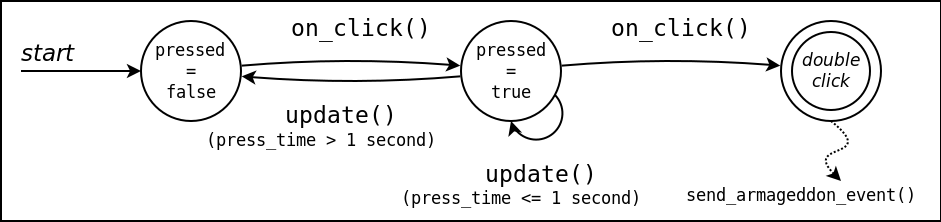
\includegraphics[width=\columnwidth]{double-click}
\caption{State machine for detecting double-clicks in the
         \emph{Armageddon button}.
\label{fig.armageddon.fsm}
}
\end{figure}

Figure~\ref{lst.armageddon}.a shows the C++ implementation for the class
\code{ArmageddonButton} with methods for rendering the button and handling
mouse and timer events.
The code in the figure focus on the double click detection and hides unrelated
parts with \code{<...>}.
%
The methods \code{update} (ln 14--26) and \code{on\_click} (ln 28--34) are
examples of \emph{short-lived callbacks}, which are pieces of code that execute
atomically in reaction to external input events.
The callback \code{on\_click} reacts to mouse clicks detected by the base class
\code{RectComponent} (ln 2), while the callback \code{update} continuously
reacts to the passage of time, frame by frame.
%Callbacks are short lived because they must react to input as fast as possible
%to let other callbacks execute, keeping the game with real-time responsiveness.
%
The class first initializes the variable \code{pressed} (ln 3) to track the
first click (ln 32).
It also initializes the variable \code{press\_time} (ln 4) to count the time
since the first click (ln 16--17).
If another click occurs within 1 second, the class signals the double click to
the application (ln 29--30).
Otherwise, the \code{pressed} and \code{press\_time} state variables are reset
(ln 18--21).
%
Figure~\ref{fig.armageddon.fsm} illustrates how we can model the double-click 
behavior in C++ as a state machine.
The circles represent the state of the variable \code{pressed}, and the arrows 
represent the callbacks manipulating it.
%
Note in Figure~\ref{lst.armageddon}.a how the accesses to the state variables
are spread across the entire class: the distance between the initialization of
\code{pressed} (ln  3) and the last access to it (ln 32) is over 40 lines in
the original file.
Arguably, this dispersion of code across methods makes the understanding and 
maintenance of the double-click behavior more difficult.
Also, even though the state variables are private, unrelated methods such as 
\code{draw}, which is defined in middle of the class (ln 10--12), can
potentially access them.

\CEU supports structured constructs to deal with events, aiming to eradicate
explicit manipulation of state variables for control-flow purposes.
%
In Figure~\ref{lst.armageddon}.b, the loop to detect double clicks (ln 4--10)
awaits the first click (ln 5) and then, while watching 1 second (ln 6--9),
awaits the second click (ln 7).
If the second click occurs within 1 second, the \code{break} terminates the
loop (ln 8) and the \code{emit} in sequence signals the double click to the
application (ln 12).
Otherwise, the \code{watching} block as a whole aborts after 1 second  and the
loop restarts, falling back to the first click \code{await} (ln 5).
%
Double click detection in \CEU does not rely on state variables and is entirely
self-contained in the \code{loop} body.
Also, those 7 lines of code \emph{only} detect the double click, leaving the
actual effect (ln 12) as well as all unrelated code (such as redrawing the
button) to happen outside the loop.

The \code{await} statement of \CEU allows for nested control-flow statements to
suspend execution while retaining all enclosing state alive, such as local
variables and next statement to execute.
Then, a subsequent reaction to an event resumes execution normally.
In contrast, method callbacks in object-oriented programming have a single
entry point at the top level of the class, in which only instance members
remain active between invocations.
In particular, locals and loops cannot persist across invocations.

\subsubsection{Case Study: The \emph{Bomber Action} Animation Sequence}
\label{sec.pats.fsms.2}

\begin{figure}
\centering
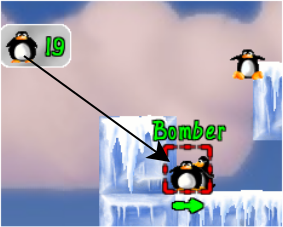
\includegraphics[width=120px]{bomber-01}
\caption{ Assigning the \emph{Bomber action} to a pingu.
\label{fig.bomber.action}
}
\end{figure}

\begin{figure}
\centering
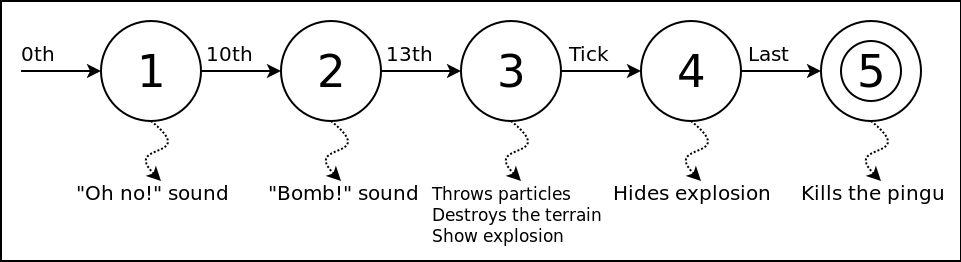
\includegraphics[width=\columnwidth]{states}
\caption{ State machine for the \emph{Bomber animation} sequence.
\label{fig.bomber.fsm}
}
\end{figure}

The player may assign actions to specific pingus, as illustrated in
Figure~\ref{fig.bomber.action}.
%
The \emph{Bomber action} explodes the clicked pingu, throwing particles around
and also destroying the terrain under its radius.%
\footnote{Bomber action animation: \url{github.com/an000/p/#2} }
%
We can model the explosion animation with a sequential state machine
(Figure~\ref{fig.bomber.fsm}) with effects associated to specific frames as
follows%
\footnote{State machine animation: \url{github.com/an000/p/#3} }:
%
\begin{enumerate}
%\setlength\itemsep{0em}
\item 0th frame:  plays a "Oh no!" sound.
\item 10th frame: plays a "Bomb!" sound.
\item 13th frame: throws particles, destroys the terrain, and shows an
                  explosion sprite.
\item Game tick:  hides the explosion sprite.
\item Last frame: kills the pingu.
\end{enumerate}

%\begin{figure}
%\centering
%\includegraphics[width=\columnwidth]{bomber-anim}
%\caption{ The \emph{Bomber action}.
%\label{fig.bomber.anim}
%}
%\end{figure}

\begin{figure*}
\begin{minipage}[t]{0.50\linewidth}
\begin{lstlisting}[numbers=right]
Bomber::Bomber (Pingu* p) :
    <...>
    spr(<...>),         // bomber sprite
    sound_ok(false),    // tracks state 2
    particle_ok(false), // tracks state 3
    colmap_ok(false),   // tracks state 3
    gfx_ok(false)       // tracks state 4
{
    <...>
    // 1. plays a "Oh no!" sound.
    play_sound("ohno");
}

void Bomber::update () {
    spr.update();
    <...>   // pingu movement

    // 2. plays a "Bomb!" sound.
    if (spr.frame()==10 && !sound_ok) {
      sound_ok = true;
      play_sound("plop");
    }

    // 3. particles, terrain, explosion sprite
    if (spr.frame()==13 && !particle_ok) {
      particle_ok = true;
      world()->get_particles()->add(...);
    }
    if (spr.frame()==13 && !colmap_ok) {
      colmap_ok = true;
      world()->remove(radius, <...>);
    }

    // 5. kills the Pingu
    if (spr.is_finished ()) {
      pingu->status(DEAD);
    }
}

void Bomber::draw (SceneContext& gc) {
    // 3. particles, terrain, explosion sprite
    // 4. tick: hides the explosion sprite
    if (spr.frame()==13 && !gfx_ok) {
      gfx_ok = true;
      gc.color().draw(explo_surf, <...>);
    }
    gc.color().draw(spr, pingu->get_pos());
}
\end{lstlisting}
\centering\small{\ax Implementation in C++}
\end{minipage}
%
\begin{minipage}[t]{0.50\linewidth}
\begin{lstlisting}[xleftmargin=2em]
code/await Bomber (void) -> ActionName
do
    <...>
    spawn Mover(); // movement in background
    var Sprite spr = spawn Sprite(<...>);
                 // frame animation in background
    watching spr do
      // 1. plays a "Oh no!" sound.
      {play_sound("ohno")};

      // 2. plays a "Bomb!" sound.
      await game.update until spr.frame==10;
      {play_sound("plop")};

      // 3. particles, terrain, explosion sprite
      await game.update until spr.frame==13;
      spawn Particles(<...>) in particles;
      call Game_Remove({&radius}, <...>);
      do
        <...>
        spawn Sprite(<...>); // explosion

        // 4. tick: hides the explosion sprite
        await game.update;
      end
      await FOREVER;
    end

    // 5. kills the pingu
    escape DEAD;
end
















.
\end{lstlisting}
\centering\small{\bx Implementation in \CEU}
\end{minipage}
%\rule{8.4cm}{0.37pt}
\caption{ The \emph{Bomber action} sequence.
\label{lst.bomber}
}
\end{figure*}

In C++, the class \code{Bomber} in Figure~\ref{lst.bomber}.a defines the
callbacks \code{draw} and \code{update} to manage the state machine of
Figure~\ref{fig.bomber.fsm}.
%
The class first defines one state variable for each effect to perform
(ln 4--7).
The ``Oh no!'' sound plays as soon as the object starts in \emph{state-1} 
(ln 11).
The \code{update} callback (ln 14--38) first updates the pingu animation and
movement on every frame, regardless of its current state (ln 15--16).
When the animation reaches the 10th frame, it switches to \emph{state-2} and
plays the ``Bomb!'' sound (ln 18--22).
The state variable \code{sound\_played} is required because the sprite frame
doesn't necessarily advance on every \code{update} invocation (e.g.,
\code{update} may execute twice during the 10th frame).
The same reasoning and technique applies to \emph{state-3} (ln 24--32 and
41--46).
The explosion sprite appears in a single frame in \emph{state-4} (ln 45).
Finally, the pingu dies after the animation frames terminate (ln 34--37).
%
Note that a single numeric state variable would suffice to track the states as
in Figure~\ref{fig.bomber.fsm}, but the original developers probably chose to
encode each state in an independent boolean 
variable to rearrange and experiment with them during development.
Still, due to the short-lived nature of callbacks, state variables are 
unavoidable and are actually the essence of object-oriented programming
(i.e., methods with mutable state).
%
Like the double click detection in C++, note that the state machine is encoded
across 3 different methods, each intermixing code with unrelated functionality
(e.g., changing frames, moving, and redrawing).

The equivalent code in \CEU for the \emph{Bomber action} in
Figure~\ref{lst.bomber}.b does not rely on state variables and reflects the
sequential state machine implicitly, using \code{await} statements to separate
the effects in direct style.
%
The \code{Bomber} is a \code{code/await} abstraction of \CEU, which is similar
to a coroutine or fiber~\cite{sync_async.cooperative}: a subroutine that
retains runtime state, such as local variables and the program counter, across
reactions to events (i.e., across \code{await} statements).
The pingu movement and sprite animation are isolated in two other
\code{code/await} abstractions and execute in separate through the \code{spawn}
primitive (ln 4--5).
%In \CEU, if multiple abstractions react to the same event, the scheduler
%employs lexical order to preserve determinism, i.e., the \code{spawn} that
%appears first in the source code reacts first~\cite{ceu.mod15}.
The event \code{game.update} (ln 12,16,24) is analogous to the \code{update}
callback of C++ and occurs on every game frame.
%
The code tracks the animation aliveness (ln 7--27) and, on termination,
performs the last bomber effect, killing the pingu (ln 30).
As soon as the animation starts, the code performs the first effect (ln 9).
The intermediate effects are performed when the corresponding conditions occur
(ln 12,16,24).
The \code{do-end} block (ln 19--25), restricts the lifespan of the
single-frame explosion sprite (ln 21): after the next game tick (ln 24), the
block terminates and automatically destroys the spawned abstraction (removing
it from the screen).
%
In contrast with the implementation in C++, all effects occur in a contiguous
chunk of code (ln 7--30), which handles no extra functionality.

\subsubsection{Summary \& Pattern Uses in Pingus}

In comparison to explicit state machines, the structured constructs of \CEU
introduce some advantages as follows:
%
\begin{itemize}
%\setlength\itemsep{0em}
\item They encode all states with direct sequential code, eliminating callbacks
      and shared state variables for control-flow purposes.
\item They handle all states (and only them) in the same contiguous block,
      improving code encapsulation.
\end{itemize}
%
Object-oriented games also adopt the \emph{state pattern} to model state
machines with subclasses describing each possible state~\cite{games.patterns}.
However, this approach is not fundamentally different from Pingus' use of
\code{switch} or \code{if} branches to decode state.

\begin{figure}
{\footnotesize
\begin{verbatim}
Action       Ceu    C++   Explicit State
---------   ----   ----   -----------------
Bomber        23     50   4 state variables
Bridger       75    100   2 state variables
Drown          6     15   1 state variable
Exiter         7     22   2 state variables
Splashed       6     19   2 state variables
\end{verbatim}
\caption{Pingus actions in \CEU and C++ in terms of \locs and state variables.
\label{tab.actions}
}
}
\end{figure}

Pingus supports 16 actions in the game.
Five of them implement at least one state machine and are considerable smaller
in \CEU in terms of \locs (Figure~\ref{tab.actions}).
%(after eliminating the state variables).
%
For the other 11 actions without state machines, the reduction in \locs is
negligible.
%
This asymmetry illustrates the gains in expressiveness when describing state
machines in direct style.

%As other examples, detecting mouse dragging in the scenario and in the small
%map to move the game viewport also involves state machines.
%State machines also appear in the \emph{FPS counter} and in UI widgets with
%visual feedback.

Among all 65 implementation files in \CEU, we found 29 cases in 25 files that
use structured mechanisms to substitute states machines.
They typically manifest as \code{await} statements in sequence (e.g.,
ln 5,7 in Figure~\ref{lst.armageddon} and ln 12,16,24 in
Figure~\ref{lst.bomber}).
%or in aborting constructs such as \code{par/or} and \code{watching}.

\subsection{Continuation Passing}
\label{sec.pats.cps}

    The completion of a long-lasting activity in the game may carry a
    continuation, i.e., some action to execute next.

\subsubsection{ Transition from \emph{Story}  to \emph{Credits} Screen}

\begin{figure*}
\begin{minipage}[t]{0.50\linewidth}
\begin{lstlisting}[numbers=right]
StoryDot::StoryDot(FileReader& reader) :
    show_credits(false), // do not show by default
{
    <...>
    reader.read("credits", show_credits);
}             // from file

void StoryDot::on_click() {
    <...>
    push(<StoryScreen>(show_credits));
    <...>
}

///

StoryScreenComp::StoryScreenComp (<...>) :
    show_credits(show_credits),
    <...>
{
    <...>
}

<...>   // draw and update page

void StoryScreenComp::next_text() {
    if (!displayed) {
      <...>
    } else {
      <...>
      if (!pages.empty()) {
        <...>
      } else {
        if (show_credits) {
          replace(<Credits>(<...>));
        } else {
          pop();
        }
      }
    }
}
\end{lstlisting}
\centering\small{\ax Implementation in C++}
\end{minipage}
%
\begin{minipage}[t]{0.50\linewidth}
\begin{lstlisting}[xleftmargin=2em]
loop do
    var int ret = await Worldmap();
    if ret==CREDITS or ret==BACK then
      <...>
      var bool is_click = await Story();
      if is_click and ret==CREDITS then
        <...>
        await Credits();
      end
    else
      <...>
    end
end


























.
\end{lstlisting}
\centering\small{\bx Implementation in \CEU}
\end{minipage}
%\rule{8.4cm}{0.37pt}
\caption{ Transition from \emph{Story} to \emph{Credits screen}.
\label{lst.story}
}
\end{figure*}

The campaign world map has clickable blue dots in the two extremes of the
map road to show introductory and closing ambience stories, respectively.
For introductory stories, the game returns to the world map after showing 
the story pages.
For closing stories, the game also shows a \emph{Credits screen} before
returning to the world map.%
\footnote{Credits screen animation: \url{github.com/an000/p/#4} }

In C++, the class \code{StoryDot} in Figure~\ref{lst.story}.a (ln 1--12) first
reads the level file (ln 5) to check whether it is a closing story and should,
after termination, show the \emph{Credits screen}.
%
The boolean variable \code{show\_credits} (ln 2,5,10) is passed to the class
\code{StoryScreen} (ln 10) and represents the screen continuation, i.e., what
to do after showing the story.
The class \code{StoryScreen} (not shown) then forwards the continuation even
further to the auxiliary class \code{StoryScreenComp} (ln 16--40).
%
When the method \code{next\_text} has no story pages left to display
(ln 32--38), it decides where to go next, depending on the continuation flag
\code{show\_credits} (ln 33).

In \CEU, the \code{loop} of Figure~\ref{lst.story}.b controls the flow between
the screens to show as a direct sequence of statements.
%
We first invoke the \code{Worldmap} (ln 2), which shows the map and lets
the player interact with it (e.g., walking around) until a dot is clicked.
If the player selects a story dot (ln 4--9), we invoke the \code{Story}
and await its termination (ln 5).
After showing the story, we check the returned values (ln 6) to perhaps show
the \code{Credits} screen (ln 8).
The enclosing loop restores the \code{Worldmap} and repeats the process.

\begin{figure*}
\centering
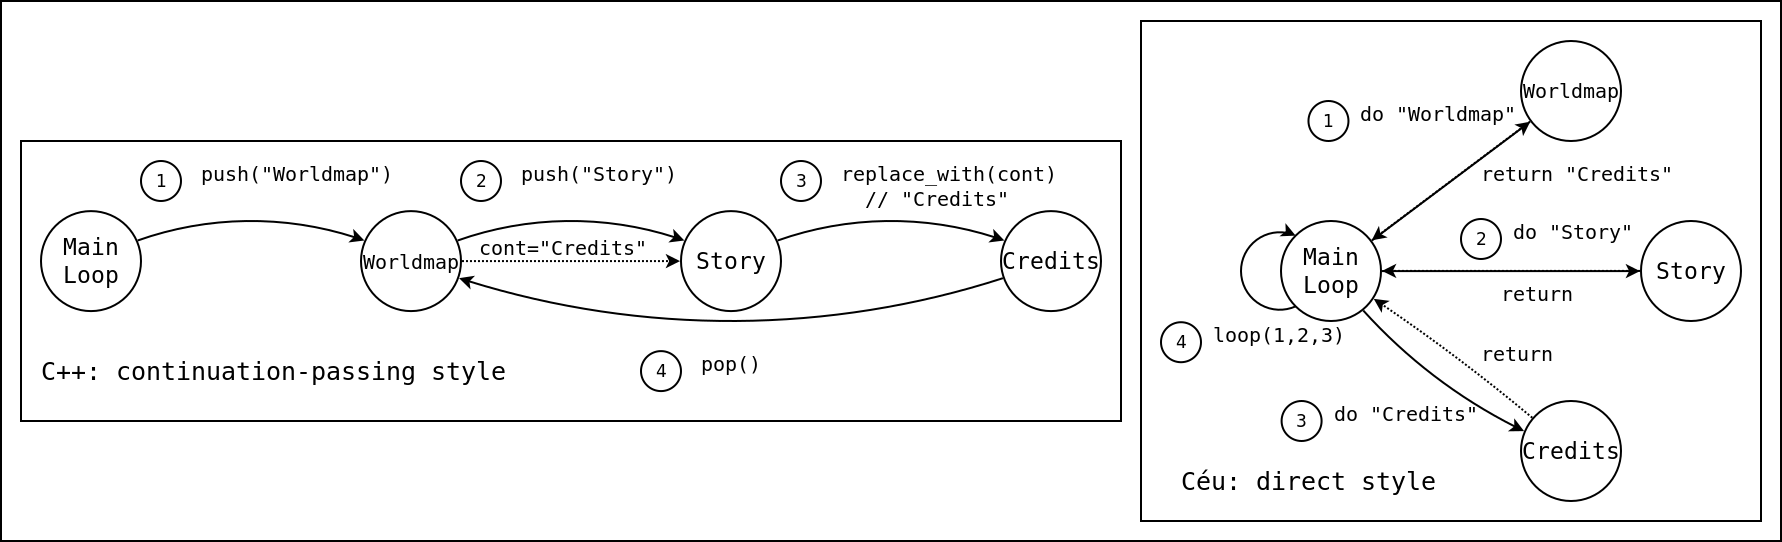
\includegraphics[width=\textwidth]{continuation}
\caption{ Continuation (C++) vs Direct (\CEU) Styles.
\label{fig.story}
}
\end{figure*}

Figure~\ref{fig.story} illustrates the \emph{continuation-passing style} of
C++ and the \emph{direct style} of \CEU for screen transitions:

\begin{enumerate}
%\setlength\itemsep{0em}
\item \code{Main Loop} $\longrightarrow$ \code{Worldmap}:
    \begin{itemize}
    %\setlength\itemsep{0em}
    \item C++ uses an explicit stack to push the \code{Worldmap} screen (not
          shown in Figure~\ref{lst.story}.a).
    \item \CEU invokes the \code{Worldmap} screen expecting a return value
          (Figure~\ref{lst.story}.b, ln 2).
    \end{itemize}
\item \code{Worldmap} (\emph{blue dot click}) $\longrightarrow$ \code{Story}:
    \begin{itemize}
    %\setlength\itemsep{0em}
    \item C++ pushes the \code{Story} screen passing the continuation flag
          (Figure~\ref{lst.story}.a, ln 10).
    \item \CEU stores the \code{Worldmap} return value and invokes the \code{Story} screen
          (Figure~\ref{lst.story}.b, ln 2,5).
    \end{itemize}
\item \code{Story} $\longrightarrow$ \code{Credits}:
    \begin{itemize}
    %\setlength\itemsep{0em}
    \item C++ replaces the current \code{Story} screen with the \code{Credits}
          screen (Figure~\ref{lst.story}.a, ln 34).
    \item \CEU invokes the \code{Credits} screen after the \code{await Story}
          returns (Figure~\ref{lst.story}.b, ln 8).
    \end{itemize}
\item \code{Credits} $\longrightarrow$ \code{Worldmap}:
    \begin{itemize}
    %\setlength\itemsep{0em}
    \item C++ pops the \code{Credits} screen, going back to the \code{Worldmap}
          screen (not shown in Figure~\ref{lst.story}.a).
    \item \CEU uses an enclosing \code{loop} to restart the process
          (Figure~\ref{lst.story}.b, ln 1--13).
    \end{itemize}
\end{enumerate}

In contrast with C++, the screens in \CEU are decoupled from each other and
only the \code{Main Loop} touches them: the \code{Worldmap} has no references
to \code{Story}, which has no references to \code{Credits}.
Changing the screen arrangements is a matter of adjusting the main loop only.

\subsubsection{Summary \& Pattern Uses in Pingus}

The direct style of \CEU has some advantages in comparison to the 
continuation-passing style of C++:
%
\begin{itemize}
%\setlength\itemsep{0em}
\item It uses structured control flow (i.e., sequences and loops) instead of 
      explicit data structures (e.g., stacks) and continuation variables (e.g.
      boolean flags).
\item The activities in sequence are decoupled and do not hold references to
      one another. % TODO: esta no outro exemplo
\item A single parent class describes the flow between the activities in a 
      self-contained block of code. % TODO: esta no outro exemplo
\end{itemize}

Continuation passing typically controls the overall structure of the game in
C++, such as screen transitions in menus and level progressions.
%
\CEU adopts the direct style technique in five cases involving screen
transitions:
the main menu, the level menu, the level set menu, the world map loop, and
the gameplay loop.
%
It also uses the same technique for the loop that switches between pingu
actions during gameplay (e.g., \emph{walking} to \emph{falling} and back to
\emph{walking}).

\subsection{Dispatching Hierarchies}
\label{sec.pats.dispatching}

    Entities form a dispatching hierarchy in which a container that receives a
    stimulus automatically forwards it to its managed children.

\subsubsection{Case Study: \emph{Bomber Action} \Code{draw} and \Code{update} Dispatching}

\begin{figure*}
\begin{minipage}[t]{0.50\linewidth}
\begin{lstlisting}[numbers=right]
class Bomber : public Action {
    <...>
    Sprite sprite;
}

Bomber::Bomber (<...>) : <...> {
    sprite.load(<...>);
    <...>
}

void Bomber::update () {
    sprite.update();
}

void Bomber::draw () {
    <...>
    sprite.draw();
}
\end{lstlisting}
\centering\small{\ax Implementation in C++}
\end{minipage}
%
\begin{minipage}[t]{0.50\linewidth}
\begin{lstlisting}[xleftmargin=2em]
code/await Bomber (void) -> ActionName do
    <...>
    var Sprite sprite = spawn Sprite(<...>);
    <...>
end












.
\end{lstlisting}
\centering\small{\bx Implementation in \CEU}
\end{minipage}
%\rule{8.4cm}{0.37pt}
\caption{ \emph{Bomber action} \code{draw} and \code{update} dispatching.
\label{lst.hier}
}
\end{figure*}

\begin{figure*}
\centering
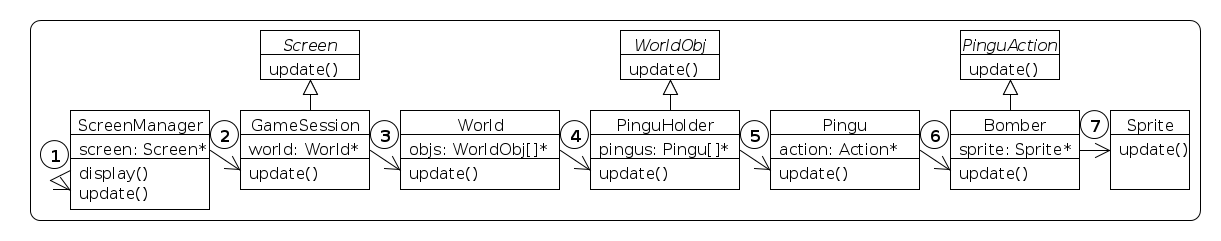
\includegraphics[width=\textwidth]{hierarchy}
\caption{Dispatching chain for \code{update}.
\label{fig.hier}
}
\end{figure*}

In C++, the class \code{Bomber} in Figure~\ref{lst.hier}.a declares a
\code{sprite} member (ln 3) to handle its animation frames.
%
The \code{Sprite} class is part of the game engine and knows how to update and
render itself.
However, the \code{Bomber} still has to respond to \code{update} and
\code{draw} requests from the game and forward them to the sprite
(ln 11--13 and 15--18).
%
To understand how the \code{update} callback flows from the original
environment stimulus to the game down to the sprite, we need to follow a long
chain of 7 method dispatches (Figure~\ref{fig.hier}):
%
\begin{enumerate}
%\setlength\itemsep{0em}
\item \code{ScreenManager::display} in the main game loop calls\\
      \code{ScreenManager::update} when starting a new frame.
\item \code{ScreenManager::update} calls \code{screen->update} for the active
      game screen (i.e., a \code{GameSession} instance, considering the screen
      in which the \code{Bomber} appears).
\item \code{GameSession::update} calls \code{world->update}.
\item \code{World::update} calls \code{objs->update} for each object in the
      world.
\item \code{PinguHolder::update} calls \code{pingu->update} for each pingu
      alive.
\item \code{Pingu::update} calls \code{action->update} for the active pingu
      action.
\item \code{Bomber::update} calls \code{sprite.update}.
      \code{Sprite::update} finally updates the animation frame.
\end{enumerate}
%
Each dispatching step in the chain is indeed necessary considering the game
architecture:
%
\begin{itemize}
%\setlength\itemsep{0em}
\item With a single assignment to \code{screen}, one can easily deactivate the
current screen and redirect all dispatches to a new screen (step 2).
\item The \code{World} class manages and dispatches events to all game
      entities with a common interface \code{WorldObj}, such as the pingus and
      traps (step 4).
\item Since it is common to iterate only over the pingus (vs. all world
      objects), the container \code{PinguHolder} manages all pingus (step 5).
\item Since a single pingu can change its actions during lifetime, the
      \code{action} member decouples them with another level of indirection
      (step 6).
\item Sprites are part of the game engine and are reusable everywhere (e.g., UI
      buttons, world objects, etc.), so it is also convenient to decouple them
      from actions (step 7).
\end{itemize}
%
Like \code{update}, the \code{draw} callback also flows through a similar
dispatching hierarchy until reaching the \code{Sprite} class.

In \CEU, the \code{Bomber} abstraction presented in Figure~\ref{lst.hier}.b
spawns a \code{Sprite} animation instance on its body (ln 3).
%
The \code{Sprite} abstraction can react directly to external \code{update}
and \code{draw} events, bypassing the program hierarchy entirely.
Events in \CEU are broadcasted to the entire application in lexical order,
i.e., an abstraction that appears first in the source code (e.g., ln 3) reacts
before another one that appears second (e.g., hidden in ln 4).
%As discussed in Section~\ref{sec.pats.fsms.2}
This rule preserves determinism and also conforms to the program static
hierarchy.
While (\emph{and only while}) the bomber abstraction is alive, the sprite
animation remains alive and reacts to the \code{update} and \code{draw} events.
The radical decoupling between the program hierarchy and reactions to events
eliminates dispatching chains entirely.
% TODO: hidden in the language runtime
%Note that one can still declare a local event to restrict its visibility like
%a local variable.

\subsubsection{Summary \& Pattern Uses in Pingus}

Passive entities subjected to hierarchies require a dispatching architecture
that makes the reasoning about the program harder:

\begin{itemize}
%\setlength\itemsep{0em}
\item The full dispatching chain may go through dozens of files.
\item The dispatching chain may interleave between classes specific to the game
      and also classes from the game engine (possibly third-party classes).
\end{itemize}

In C++, the update subsystem touches 39 files with around 100 lines of code
just to forward \code{update} methods through the dispatching hierarchy.
For the drawing subsystem, 50 files with around 300 lines of code.
The implementation in C++ also relies on dispatching hierarchy for
\code{resize} callbacks, touching 12 files with around 100 lines of code.
%
Most of this code is eliminated in \CEU since abstractions can react directly
to the environment, not depending on hierarchies spread across multiple files.

Note that dispatching hierarchies cross game engine code, suggesting that most
games also rely heavily on this control-flow pattern.
In the case of the Pingus engine, we rewrote 9 files with a reduction from 515
to 173 \locs (not listed in Figure~\ref{tab.tree}), mostly due to dispatching
code removal.

\subsection{Lifespan Hierarchies}
\label{sec.pats.lifespan}

    Entities form a lifespan hierarchy in which a terminating container entity
    automatically destroys its managed children.

\subsubsection{Case Study: Static Game UI Widgets}

\begin{figure}
\centering
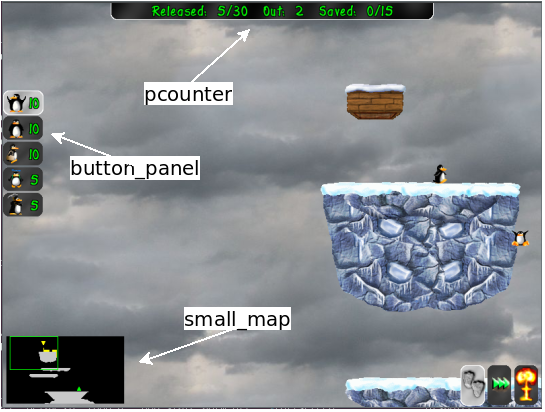
\includegraphics[width=\columnwidth]{game-session-arrows}
\caption{UI children with static lifespan.
\label{fig.ui}
}
\end{figure}

Figure~\ref{fig.ui} shows the game UI widgets with action buttons, score
counters, and a small map, all coexisting with the game screen during its
whole lifespan.

\begin{figure*}
\begin{minipage}[t]{0.50\linewidth}
\begin{lstlisting}[numbers=right]
GameSession::GameSession(<...>) :
    <...>
{
    <...>    // these widgets are always active...
    btpanel  = new ButtonPanel(<...>);
    pcounter = new PingusCounter(<...>);
    smallmap = new SmallMap(<...>);
    <...>
    uimgr->add(btpanel);  // ...but are added
    uimgr->add(pcounter); //  dynamically to the
    uimgr->add(smallmap); //  dispatching hierarchy
    <...>
}
\end{lstlisting}
\centering\small{\ax Implementation in C++}
\end{minipage}
%
\begin{minipage}[t]{0.50\linewidth}
\begin{lstlisting}[xleftmargin=2em]
code/await Game (void) do
    <...> // other coexisting functionality
    spawn ButtonPanel(<...>);
    spawn PingusCounter(<...>);
    spawn SmallMap(<...>);
    <...> // other coexisting functionality
end





.
\end{lstlisting}
\centering\small{\bx Implementation in \CEU}
\end{minipage}
%\rule{8.4cm}{0.37pt}
\caption{ Managing the UI widgets lifecycle.
\label{lst.ui}
}
\end{figure*}

In C++, the widgets are created in the constructor of the class
\code{GameSession} in Figure~\ref{lst.ui}.a (ln 5--7), added to a UI container
(ln 9--11), and are never removed since they must always be visible.
Arguably, to better express the intent of making them coexist with the game
screen, the widgets could alternatively be declared as top-level automatic
(non-dynamic) members.
However, the class relies on a container to automate \code{draw} and
\code{update} dispatching to the widgets, as discussed in
Section~\ref{sec.pats.dispatching}.
The container method \code{add} expects only dynamically allocated children
because they are automatically deallocated inside the container destructor.
%
However, the dynamic nature of containers in C++ demand extra caution from
programmers:
%
\begin{itemize}
%\setlength\itemsep{0em}
\item When containers are part of a dispatching chain, it gets even harder to
      know which objects are dispatched at a given moment:
      one has to ``simulate'' the program execution and track calls to
      \code{add} and \code{remove}.
\item For objects with dynamic lifespan, calls to \code{add} must always have
      matching calls to \code{remove}:
      missing calls to \code{remove} lead to memory and CPU leaks (to be
      discussed as the \emph{lapsed listener problem} in
      Section~\ref{sec.pats.lifespan.2}).
\end{itemize}

In \CEU, the UI entities that coexist are simply created in the same lexical
block of the \code{Game} abstraction in Figure~\ref{lst.ui}.b (ln 3--5).
%
Since abstractions can react independently, they do not require a dispatching
container.
%
Lexical lifespan never requires containers, allocation and deallocation, or
explicit references.
In addition, all required memory is known at compile time, similarly to
stack-allocated local variables.
%
The \emph{Bomber action} of Section~\ref{sec.pats.fsms.2} also relies on
lexical scope to delimit the lifespan of the explosion sprite into a single
frame (Figure~\ref{lst.bomber}, ln 19--25).

\subsubsection{Case Study: Dynamic Pingus Lifecycle}
\label{sec.pats.lifespan.2}

%\begin{figure}
%\centering
%\includegraphics[width=\columnwidth]{pingus_create_die-anim}
%\caption{Creation and death of pingus.
%\label{fig.pingus_create_die}
%}
%\end{figure}

A pingu is a dynamic entity created periodically and destroyed under certain
conditions, such as falling from a high altitude.%
\footnote{Death of pingus animation: \url{github.com/an000/p/#5} }
%

\begin{figure*}
\begin{minipage}[t]{0.50\linewidth}
\begin{lstlisting}[numbers=right]
Pingu* PinguHolder::create_pingu (<...>) {
    <...>
    Pingu* pingu = new Pingu (<...>);
    pingus.push_back(pingu);
    <...>
}

void PinguHolder::update() {
    <...>
    while(pingu != pingus.end()) {
      (*pingu)->update();
      if ((*pingu)->status() == DEAD) {
        pingu = pingus.remove(pingu);
      }
      <...>
      ++pingu;
    }
}

.
\end{lstlisting}
\centering\small{\ax Implementation in C++}
\end{minipage}
%
\begin{minipage}[t]{0.50\linewidth}
\begin{lstlisting}[xleftmargin=2em]
code/await Game (void) do
    <...>
    pool[] Pingu pingus;
    code/await Pingu_Spawn (<...>) do
      <...>
      spawn Pingu(<...>) in pingus;
    end
    <...>   // code invoking Pingu_Spawn
end

code/await Pingu (<...>) do
    <...>
    loop do
      await game.update;
      if Pingu_Is_Out_Of_Screen() then
        <...>
        escape PS_DEAD;
      end
    end
end
\end{lstlisting}
\centering\small{\bx Implementation in \CEU}
\end{minipage}
%\rule{8.4cm}{0.37pt}
\caption{ Managing the pingus lifecycle.
\label{lst.pingus}
}
\end{figure*}

In C++, the class \code{PinguHolder} in Figure~\ref{lst.pingus}.a is a
container that holds all alive pingus.
%
The method \code{PinguHolder::create\_pingu} (ln 1--6) is called periodically
to create a new \code{Pingu} and add it to the \code{pingus} collection
(ln 3--4).
The method \code{PinguHolder::update} (ln 8--18) checks the state of all
pingus on every frame, removing those with the dead status (ln 12--14).
%
Note that if the programmer disregards the call to \code{remove}, a dead pingu
would remain in the collection and still update on every frame (ln 11).
Since the \code{draw} behavior for a dead pingu is innocuous, the death could
go unnoticed when testing it but the program would keep consuming memory and
CPU time.
%
This problem is known as the \emph{lapsed listener}~\cite{games.patterns} and
also occurs in languages with garbage collection:
a container typically holds a strong reference to a child (sometimes the only 
reference to it), and the runtime cannot magically detect it as garbage.
%
Hence, entities with dynamic lifespan always require explicit matching
\code{add} and \code{remove} calls associated to a container (ln 4,13).

\begin{figure}
\centering
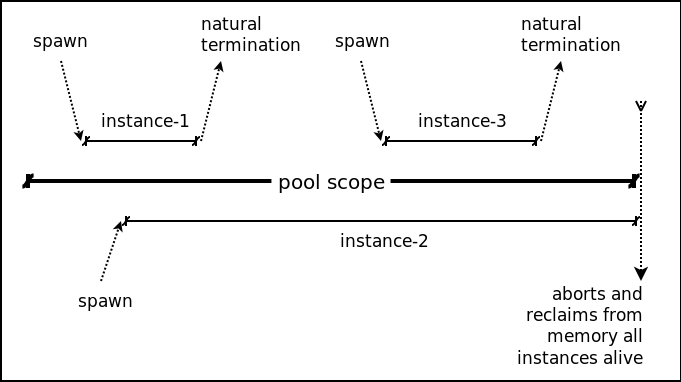
\includegraphics[width=\columnwidth]{pool}
\caption{Lifespan of dynamic instances.
\label{fig.pool}
}
\end{figure}

\CEU supports \code{pool} declarations to hold dynamic abstraction instances.
In addition, the \code{spawn} statement supports a pool identifier to associate
a new instance with a pool.
%
The game screen in Figure~\ref{lst.pingus}.b spawns a new \code{Pingu} on every
invocation of \code{Pingu\_Spawn} (ln 4--7).
%
The \code{spawn} statement (ln 6) specifies the pool declared at the top-level
block of the game screen (ln 3).
In this case, the lifespan of the new instances follows the scope of the pool
(ln 1--9) instead of the enclosing scope of the \code{spawn} statement
(ln 4--7), surviving the call to \code{Pingu\_Spawn}.
Since pools are also subject to lexical scope, the lifespan of all dynamically
allocated pingus is constrained to the game screen.
%
Lexical scopes handle memory and event dispatching automatically for static
instances and also for pools.
However, the lifespan of a dynamic instance does not necessarily have to match
the lifespan of its associated pool (Figure~\ref{fig.pool}).
In \CEU, when the execution block of a dynamic instance terminates, which
characterizes its \emph{natural termination}, the instance is automatically
removed from its pool.
Therefore, dynamic instances do not require any extra bookkeeping related to 
containers or explicit deallocation.
%
To remove a pingu from the game in \CEU, we just need to terminate its execution
block according to the appropriate conditions:
%
The \code{escape} statement (ln 17) aborts the execution block of the
\code{Pingu} instance, removing it from its associated pool automatically.
Hence, a dynamic instance that terminates naturally leaves no traces in the 
program.

\subsubsection{Summary \& Pattern Uses in Pingus}

Lexical lifespan for static instances and natural termination for dynamic
instances provide some advantages in comparison to lifespan hierarchies through
containers:

\begin{itemize}
%\setlength\itemsep{0em}
\item Lexical scope makes an abstraction lifespan explicit in the source code.
      All entities in a game have an associated lexical lifespan.
\item The memory for static instances is known at compile time.
\item Natural termination makes an instance innocuous and, hence, susceptible
      to immediate reclamation.
\item Instances (static or dynamic) never require explicit manipulation of
      pointers/references.
\end{itemize}

The implementation in \CEU has over 200 static instantiations spread across all
65 files.
For dynamic entities, it defines 23 pools in 10 files, with almost 96
instantiations across 37 files.
Pools are used to hold explosion particles, levels and level sets loaded from
files, gameplay \& worldmap objects, and also UI widgets.

\section{Related Work}
\label{sec.related}

The control-flow patterns presented in this paper closely relate to the
\emph{GoF} behavioral patterns~\cite{gof}, which are discussed in the context
of video games in previous
work~\cite{games.patterns,games.gof.2015,games.gof.2007}.
%
The original Pingus in C++ uses variations of the patterns
    \emph{state} (Sections~\ref{sec.pats.fsms} and \ref{sec.pats.cps}),
    \emph{visitor} (Sections~\ref{sec.pats.dispatching}~and~\ref{sec.pats.lifespan}), and
    \emph{observer} (to handle events in general)
as implementation techniques to achieve the desired higher-level
control-flow patterns described in the paper.
%
\CEU overcomes the need of behavioral patterns with support, at the language
level, for structured control-flow mechanisms and event-based communication via
broadcast.
%
%As an example, the \emph{state pattern} for the bomber animation in C++ in
%Section~\ref{sec.pats.fsms} becomes a series of blocks separated by
%\code{await} statements in \CEU.

A number of domain-specific languages, frameworks, and techniques have been
proposed for particular subsystems of the game logic, such as
animations~\cite{games.anims.2006,games.anims.2003,games.anims.1996,games.anims.1982},
game state and screen progression~\cite{games.fsms.2006.1,games.fsms.2006.2}, and
behavior and AI modeling~\cite{games.bts,games.bts.unreal}.
%
In Pingus, the adoption of \CEU is not restricted to a specific subsystem.
We employed \CEU at the very core of the game for event dispatching
(Section~\ref{sec.pats.dispatching}) and memory management of entities
(Section~\ref{sec.pats.lifespan}), eliminating parts of the original game
engine.
We also implemented all entity animations and behaviors
(Section~\ref{sec.pats.fsms}), and screen transitions
(Section~\ref{sec.pats.cps})
%, and intermodule communication (Section~\ref{sec.pats.signaling})
using the available control mechanisms of \CEU.
%
Furthermore, \CEU is a superset of C targeting reactive systems in general, not
only games, and has also been successfully adopted in other domains, such as
    wireless sensor networks~\cite{ceu.sensys13,ceu.terra} and
    multimedia systems~\cite{ceumedia.webmedia16}.

Functional reactive programming (FRP)~\cite{frp.fran} contrasts with
structured synchronous reactive programming (SSRP) as a complementary
programming style for reactive applications.
%
We believe that FRP is more suitable for data-intensive applications, while 
SSRP, for control-intensive applications.
%
On the one hand, FRP uses declarative formulas to specify continuous functions 
over time, such as for physics or data constraints among entities.
%
On the other hand, describing a sequence of steps or control-flow dependencies
in FRP requires to encode explicit state machines so that functions can switch
behavior depending on the current state.
%
FRP has been successfully used to implement a 3D first person shooting game
from scratch, but with some performance considerations~\cite{games.frag}.
%
%Instead, we rewrote an existing game and did it in small steps while keeping it
%working.
Although we do not provide a performance evaluation (Pingus is not performance
sensitive), existing work on \CEU shows that it is comparable to C in the
context of embedded systems~\cite{ceu.sensys13}.
Nonetheless, given the tight integration between \CEU and C/C++, critical parts
of games can be preserved in C++ if needed.

\section{Conclusion}
\label{sec.conclusion}

We advocate \emph{Structured Synchronous Reactive Programming} as a productive
alternative for game logic development.
%
We use the video game \emph{Pingus} as a qualitative case study.
We compare the implementation of six game behaviors in C++ and \CEU and discuss
how structured reactive mechanisms can eliminate callbacks and let programmers
write code in direct style.
%
Ultimately, we rewrote about 1/4 of the whole codebase (9.186 from 39.362 lines
of code) which comprises the core of the game logic that is susceptible to
structured reactive programming.
%We employed a \emph{live code rewrite}, i.e., starting from the original
%codebase in C++, we reimplemented it piece-by-piece in \CEU without breaking
%the game compilation and execution.

We categorize the behaviors in four recurrent control-flow patterns:
%
\emph{State machines} are the workhorses of the game logic, appearing in
animations, AI behaviors, and input handling.
\CEU can encode states implicitly with sequential statements,
% in the same contiguous block,
eliminating shared state variables and improving code encapsulation.
%
\emph{Continuation passing} controls the overall structure of the game, such as
screen transitions and level progressions.
Similarly to state machines, \CEU describes the flow of the game as sequential
statements in self-contained blocks, eliminating explicit data structures and
continuation variables.
%spread across multiple classes (e.g., stacks and boolean flags).
%decouple activities by
%
\emph{Dispatching hierarchies} disseminate input events through the game
entities and serve as a broadcast communication mechanism.
Event broadcasting is at the core of the semantics of \CEU, allowing entities
to react directly to inputs and bypass the program hierarchy entirely.
%In C++, a considerable amount of interleaving code in the game logic and
%engine is just destined to event dispatching.
%
\emph{Lifespan hierarchies} manage the memory and visibility of game entities
through class fields and containers.
In \CEU, all entities have an associated lexical scope, similarly to local
variables with automatic memory management.
%This reduces explicit manipulation of pointers and references considerably.

Overall, we most difficulties in implementing control-flow behavior in game
logic is not inherent to this domain, but a result of accidental complexity due
to the lack of structured abstractions and an appropriate concurrency model to
develop event-based applications.

\begin{comment}
\section*{Acknowledgments}

The authors would like to thank Leonardo Kaplan and Alexander Tkachov for early
explorations and prototypes of the game rewrite.
\end{comment}

\newpage
\bibliographystyle{cag-num-names}
\bibliography{my,other}

\end{document}
